\documentclass[preview,border=5pt]{standalone}
\usepackage{teaching}
\begin{document}

\centering

\begin{tikzpicture}[yscale=2,xscale=1,scale=0.5,inner sep=0.3mm, label distance=1.5mm]

\node(t) at (0,1) {\Large $y = mx + c$};
\draw[->] (0,0.5) -- (0,-0.2);
\node(t) at (0,-1) {\Large $x = \dfrac{y-c}{m}$};

\end{tikzpicture}

\end{document}